%*******************************************************************************
%*********************************** First Chapter *****************************
%*******************************************************************************

\chapter{Introduction}
\label{chap:introduction}

Vision is one of the most important senses that humans possess. It is an amazing process of how the eyes and brain translate light waves into interpreted images of our surroundings. Reflected light waves from objects are bent, or refracted, when passing through the cornea, then bent again passing through the lens and eventually hits the retina. The image is translated into impulses that travels to the brain, more specifically the occipital lobe, through the optic nerve such that the image can be interpreted. The shape of eyes affect how we things in the world are seen and kept in focus. For people with normal vision, the light waves hits the retina at the focal point where the light waves coincide. However, the eyes are longer for nearsighted eyes which moves the focal point closer to the lens such that the light waves are more spread out across the retina. For farsighted people, the eyes are shorter which moves the focal point behind the retina. Luckily, the position of the focal point can be corrected for both near- and farsighted eyes by placing a concave and convex lens respectively in front of the eyes, e.g., by using eyeglasses. However, there exist many severe cases of low vision where not even eyeglasses can help where other kinds of help is necessary for assisting the people in situations where vision is a necessity. 

There exist many different types of aids and assistive tools for helping visually impaired people (VIP) in their daily lives. A very common aid is the white cane used for enhancing the mobility of VIPs by extending their touch to prepare the users for what is ahead of them. There also exists many electronic devices, e.g., screen readers and Braille typewriter machines, that have enabled VIPs to have near-equal opportunities for office work. More recently, several computer vision-based assistive vision tools have emerged in the form of wearable devices and mobile applications for helping with, e.g., reading printed documents and bar codes for item recognition. However, computer vision-based systems can face several challenges when deployed in the real world which makes their recognition performance suffer. Therefore, there is a necessity for developing computer vision methods that perform various kinds of recognition tasks in a robust and time-efficient manner. 

Despite the immense successes in computer vision in recent years, why is computer vision difficult to perform in real-world settings? One part of the reason is that it is very challenging to specify a model of the visual world that has been injected with knowledge about the rich complexity that can exist in images~\cite{szeliski2010computer}. Interestingly, tasks that are seemingly simple for humans, such as the differences between apples and pears, can be difficult for computers. A popular approach for enabling computers to learn various concepts is machine learning where the computer learns a model of some phenomena from large sets of examples. The approach of learning from data and experiences has been shown across various tasks~\cite{akkaya2019solving, brown2020language, silver2016mastering} other than computer vision to be more efficient than relying on hard-coded knowledge for solving decision-making problems. However, collecting large sets of data is often time-consuming and labor-intensive which makes it challenging to deploy machine learning systems in the real-world where data is even more expensive to collect. Without overcoming the challenge of data collection, we need to develop data-efficient methods that can learn from few examples and generalize to new scenarios for enabling computer vision-based assistive vision devices to be useful for VIPs.   



\MK{ 
\begin{itemize}
	\item the connection between all papers is image classification
	\item talk about how complex the visual system is and how computer vision is used to replicate this
	\item talk about the challenges that can arise without having visual capabilities so that using computer vision would help, for example finding lost items at home
\end{itemize}
}


\section{Vision Impairments}
There are many different degrees of vision impairments ranging from problems with seeing from near or farther distances to blindness. Vision impairments are generally assessed by measuring the visual acuity from a fixed distance~\cite{who2019world}. In 2020, the World Health Organization (WHO) estimated that at least 2.2 billion people live with a near or distance vision impairment, wherein at least 1 billion cases the impairments could have been prevented or yet has to be addressed~\cite{who2019world}. The untreated cases are projected to grow to 1.7 billion people by 2050 mainly due to population growth and aging~\cite{bourne2021trends}. The leading causes for vision loss are uncorrected refractive errors (161 million people with distance vision loss and 510 million people with near vision loss), untreated cataracts (100 million people), age-related macular degenerationm (8.1 million), glaucoma (7.8 million), diabetic retinopathy (4.4 million) where 90\% of vision losses are preventable and treatable~\cite{steinmetz2021causes}. Furthermore, the prevalence of distance vision impairment are estimated to be four times higher in low- and middle-income regions than in high-income regions~\cite{steinmetz2021causes}.  

Several kinds of aids and tools have been developed for VIs to facilitate their capabilities of performing everyday tasks.   


%In Sweden, there are over 100.000 people with 




In 2020, there were almost 600 million people with mild to severe visual impairments around the world~\cite{bourne2021trends}. 

Describe common causes for visual impairment. What aids are there for helping them out, which will lead to assistive vision devices in the next section. 

Challenges: Mobility related challenges are what the VIs are most concerned about in general~\cite{stahl2018levnadsundersokning}.

VIPs that had to change their careers due to inaccessible apps and systems at their workplace~\cite{gotesson2019challenges, gotesson2019utmaningar}. Conclusion was that VIPs should be involved in the development and design process of such products, and that this should be included when educating User Experience (UX) designers. 


\section{Assistive Technologies Based on Computer Vision} %\section{Object Recognition for Assistive Vision}

Describe research and commercial products that uses computer vision-based assistive devices. Discuss challenges with those devices, e.g. getting real data, how to train them more data-efficiently, and how to learn new classes, which will lead to my contributions later. 

\cite{manduchi2012computer} highlights the current state of affairs, challenges, and potential outcomes of electronic devices for assistive vision. 

\section{Scope of Thesis}
Discuss how thesis is narrowed down and focused on image classification and like data collection, how to use additional labels, and then how to learn new labels continuously. 


% Thesis contributions

\section{Thesis Contributions}
\label{sec:contributions}

In this section, we summarize the contributions of each of the included papers as well as briefly describing the contributions of each author to the manuscripts. 

\subsection{Paper A: A Hierarchical Grocery Store Image Dataset with Visual and Semantic Labels}
\label{sec:paperA}

\textbf{Authors:} Marcus Klasson, Cheng Zhang, Hedvig Kjellström. 

\paragraph{Summary}
We collect a dataset with natural images of raw and refrigerated grocery items taken in grocery stores in Stockholm, Sweden, for evaluating image classification models on a challenging real-world scenario. The data collection was performed by taking photos of groceries with a mobile phone to simulate a scenario of grocery shopping using an assistive vision app. Furthermore, we downloaded iconic images and text descriptions of each grocery item by web-scraping a grocery store website to enhance the dataset with information describing the semantics of each individual item. the items are grouped based on their type, e.g., apple, juice, etc., to provide the dataset with a hierarchical labeling structure. 

We provide benchmark results evaluated using pre-trained and fine-tuned CNNs for image classification. Moreover, we take an initial step towards utilizing the rich product information in the dataset by training the classifiers with representations where both natural and iconic images have been combined through a multi-view VAE. 


\paragraph{Author Contributions}
CZ and HK presented the idea and the data collection procedure for the natural images and web-scraped information. MK performed the data collection including visiting the grocery stores for taking the natural images and the web-scraping of the grocery store website for iconic images and text descriptions. MK performed all the experiments. All authors contributed to discussing the results and contributed to writing the manuscript. 


\subsection{Paper B: Using Variational Multi-View Learning for Classification of Grocery Items}
\label{sec:paperB}

\textbf{Authors:} Marcus Klasson, Cheng Zhang, Hedvig Kjellström. 

\paragraph{Summary} 
We investigate whether training image classifiers can benefit from learning joint representations of grocery items using multi-view learning over the natural images and web-scraped information of the grocery items in the Grocery Store dataset (see Paper \ref{sec:paperA}). We employ a deep multi-view model based on VAEs called Variational Canonical Correlation Analysis (VCCA)~\cite{wang2016deep} for learning joint representations of the different data types, i.e., natural images, iconic images, and text descriptions. We performed a thorough ablation study over all data types to demonstrate how they contribute individually to enhancing the classification performance. Furthermore, we apply two classification approaches where we (i) train the classifier on the joint latent representations, and (ii) using a generative classifier by incorporating a class decoder to the VCCA model that can be used for classifying images. 

We performed a thorough ablation study over all data types to demonstrate how they contribute individually to enhancing the classification performance. To gain further insights into our results, we visualized the learned representations of the grocery items from VCCA and discussed how the iconic images and text descriptions help the model to better distinguish between the groceries. Our results show that the iconic images help to group the items based on their color and shape while text descriptions separate the items based on differences in ingredients and flavor. Finally, we concluded that utilizing the iconic images and text descriptions yielded better classification results than only using natural images. 


\paragraph{Author Contributions} 
CZ and HK presented the idea and all authors contributed to formalizing the methodology. 
MK performed all the experiments and created the visualizations. 
All authors took part in discussing the results.
All authors contributed to writing the manuscript. 


\subsection{Paper C: Learn the Time to Learn: Replay Scheduling for Continual Learning}
\label{sec:paperC}

\textbf{Authors:} Marcus Klasson, Hedvig Kjellström, Cheng Zhang. 

\paragraph{Summary}
In this paper, we show that learning the time to replay different tasks can be critical for continual learning (CL) performance in replay-based methods. As the main assumption in replay-based CL is that only a small set of historical data can be re-visited for mitigating catastrophic forgetting, most works have focused on improving the sample quality of the replay memory. However, in many real-world applications, historical data is accessible at all times, e.g., by storing it on the cloud. But although all historical data could be stored, retraining machine learning systems on a daily basis is prohibitive due to processing times and operational costs. Therefore, small replay memories are still needed in CL to mitigate catastrophic forgetting when learning new tasks. To this end, we propose to learn the time to learn for a CL system, in which we learn schedules over which tasks to replay at different times. Inspired by human learning, we demonstrate that scheduling over the time to replay is critical to the final CL performance with finite memory resources. We then illustrate our idea with scheduling over which tasks to replay by learning such policy with Monte Carlo tree search. We perform extensive evaluation showing that learning replay schedules can significantly improve the performance compared to baselines without learned scheduling. We also show that our method can be combined with any replay-based method and memory selection technique. Finally, our results indicate that the learned schedules are also consistent with human learning insights.



\paragraph{Author Contributions} 
CZ presented the idea and MK and CZ contributed to formalizing the methodology. 
MK performed all the experiments. 
All authors took part in discussing the results and contributed to writing the manuscript. 


\subsection{Paper D: Meta Policy Learning for Replay Scheduling in Continual Learning}
\label{sec:paperD}

\textbf{Authors:} Marcus Klasson, Hedvig Kjellström, Cheng Zhang. 

\paragraph{Summary} 



\paragraph{Author Contributions} CZ presented the idea. 

% Thesis outline

\section{Thesis Outline}
\label{sec:outline}


\begin{comment}
Here is an example for referencing figure \ref{EnergySources}. Example of citing \cite{BP2019} and \cite{Chen2016}.
%%%%%%%%%%%%%% Figure: Energy sources
\begin{figure}[h]
	\centering
	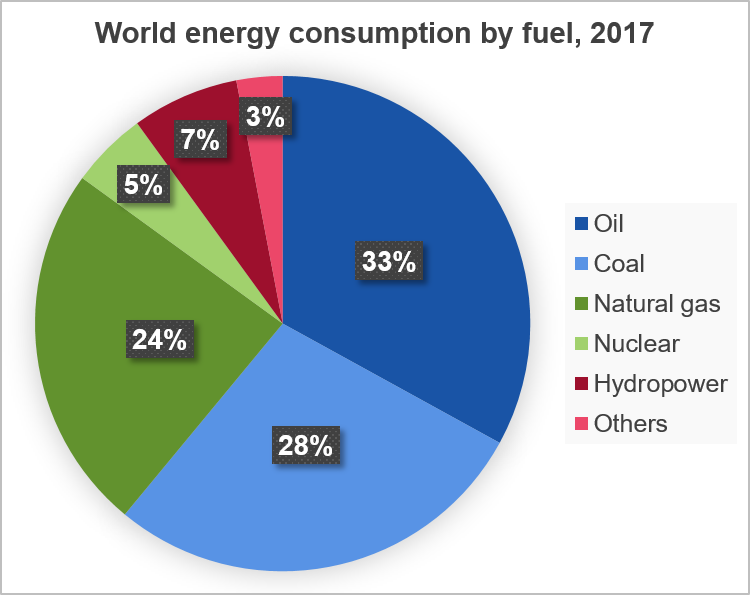
\includegraphics[scale=0.6]{Figs/Ch1_EnergySources.png}
	\caption{The world's energy consumption by fuel in 2017. }
	\label{EnergySources}
\end{figure}

%%%%%%%%%%%%%%%%%%%%%%%%%%%%%%%%%%%%%%%%
\section{Section}
Example of a table
%%%%%%%%%%%%%%%%%%%%%%%%%%%%%%%% Table: Tokamaks
\begin{table}[t!]
	\centering
	\caption{List of experimental tokamaks worldwide. Note: ITER is currently under construction and the first plasma is predicted for 2025-2028.}
	\begin{tabular}{ccccc}
		\hline
		\textbf{Name} & \textbf{Location} & \textbf{B-field} & \textbf{Major/minor radius}  \\
		\hline
		JET     & England      & 4.0 T & 3.0 m / 1.3 m \\
		ITER    & France       & 5.3 T & 6.2 m / 2.0 m \\
		AUG		& Germany      & 3.1 T & 1.7 m / 0.7 m \\
		WEST	& France	   & 3.7 T & 2.5 m / 0.5 m \\
		TCV     & Switzerland  & 1.5 T & 0.9 m / 0.3 m \\
		DIII-D  & USA          & 2.2 T & 1.7 m / 0.7 m \\
		TFTR 	& USA          & 6.0 T & 2.5 m / 0.9 m \\
		JT-60   & Japan        & 4.0 T & 3.4 m / 1.0 m \\
		K-STAR  & South Korea  & 3.5 T & 1.8 m / 0.5 m \\
		EAST    & China        & 3.5 T & 1.9 m / 0.5 m \\
		\hline
	\end{tabular}
	\label{TokamakTable}
\end{table}
\end{comment}
